% !TeX program = pdflatex
% Original architecture-engineering guidance; no licensed source text embedded.
\documentclass[11pt,letterpaper]{article}
\usepackage[T1]{fontenc}
\usepackage{lmodern,microtype}
\usepackage[margin=0.85in,headheight=16pt]{geometry}
\usepackage[table]{xcolor}
\usepackage{booktabs,tabularx,longtable,array,ragged2e}
\usepackage{tikz}
\usetikzlibrary{positioning,arrows.meta}
\usepackage{enumitem,needspace,fancyhdr,hyperref}
\definecolor{navy}{HTML}{17364D}
\definecolor{teal}{HTML}{087D83}
\definecolor{muted}{HTML}{516371}
\hypersetup{colorlinks=true,linkcolor=teal,urlcolor=teal}
\setlength{\parindent}{0pt}
\setlength{\parskip}{5pt}
\setlength{\emergencystretch}{3em}
\raggedbottom
\setlist{leftmargin=1.5em,itemsep=2pt,topsep=3pt}
\renewcommand{\arraystretch}{1.2}
\newcolumntype{Y}{>{\RaggedRight\arraybackslash}X}
\pagestyle{fancy}\fancyhf{}
\fancyhead[L]{\small\sffamily\color{navy} ARCHITECTURE ENGINEERING}
\fancyhead[R]{\small\sffamily\color{muted} SUITE / 1.0}
\fancyfoot[L]{\small\sffamily\color{muted} V\&B / ISO 42010:2022}
\fancyfoot[R]{\small\thepage}
\newcommand{\docsection}[1]{\Needspace{5\baselineskip}\section{#1}}
\newcommand{\docsub}[1]{\Needspace{4\baselineskip}\subsection{#1}}
\newcommand{\field}[1]{\par\textbf{#1}\par\noindent\rule{\linewidth}{0.3pt}\par\vspace{0.5em}}
\begin{document}
% Distinct page labels avoid duplicate Hyperref destinations after the cover.
\pagenumbering{roman}
\begin{titlepage}\thispagestyle{empty}\raggedright
\vspace*{0.65in}
{\sffamily\bfseries\color{teal} ARCHITECTURE DOCUMENTATION / METHODOLOGY\par}
\vspace{0.35in}
{\sffamily\bfseries\color{navy}\Huge Software Architecture Documentation with Views and Beyond and ISO/IEC/IEEE 42010:2022\par}
\vspace{0.2in}
{\sffamily\Large\color{muted} Principles, Viewpoints, Modeling Conventions, Architectural Traceability, and Conformance\par}
\vspace{0.35in}\noindent{\color{teal}\rule{\linewidth}{1.5pt}}\par
\vspace{0.3in}
A practical architecture documentation methodology integrating stakeholder-driven view selection with edition-specific architecture description concepts, original workflow controls, and evidence-based review.

\vfill
{\sffamily\small Edition 1.0 \quad / \quad 25 November 2026\par
Status: library working edition \quad / \quad Original engineering guidance\par}
\end{titlepage}
\pagenumbering{arabic}
\tableofcontents\clearpage
\docsection{Purpose and architectural vocabulary}
Use an architecture description (AD) to communicate architecture, not to equate a design with a document. A software architecture document (SAD) is the document-centric packaging of an AD. The entity of interest (EoI) is the subject; its environment contains interacting entities and constraints. The scope may be an existing, proposed, or reference architecture, but label the state clearly. ISO 42010 clauses 1, 3 and 5 establish the distinction; V\&B prologue P.2--P.4 supplies the practical approach.

The standard governs description obligations, not the correctness of the system, the tooling stack, or a compulsory SAD chapter order. Views and Beyond supplies a way to choose relevant structures and document their semantics. An architecture style specializes structural element and relation types; a viewpoint is a specification of conventions for addressing concerns. Neither concept is interchangeable with a system-specific view.

\begin{longtable}{@{}>{\RaggedRight\arraybackslash}p{0.457\linewidth}>{\RaggedRight\arraybackslash}p{0.457\linewidth}@{}}
\toprule
\textbf{Concept} & \textbf{Engineering use}\\\midrule
\endhead
Stakeholder & Identified party with an interest in the EoI.\\
Perspective & A way of considering the EoI; associate holders, concerns and covering viewpoints.\\
Concern & Question or matter important to identified stakeholders.\\
Aspect & Character of the EoI relevant to concerns; structural, behavioral, informational, etc.\\
Viewpoint & Versioned conventions for constructing, interpreting and using views.\\
View / view component & System-specific information; components can be modeled or documented with a legend.\\
Model kind / legend & Reusable model conventions / interpretation guidance.\\
Correspondence / method & Recorded relation / governing means to establish or assess that relation.\\
Decision / rationale & Consequential architectural choice and its justification.\\
\bottomrule
\end{longtable}
\docsection{Integrated workflow}
\begin{center}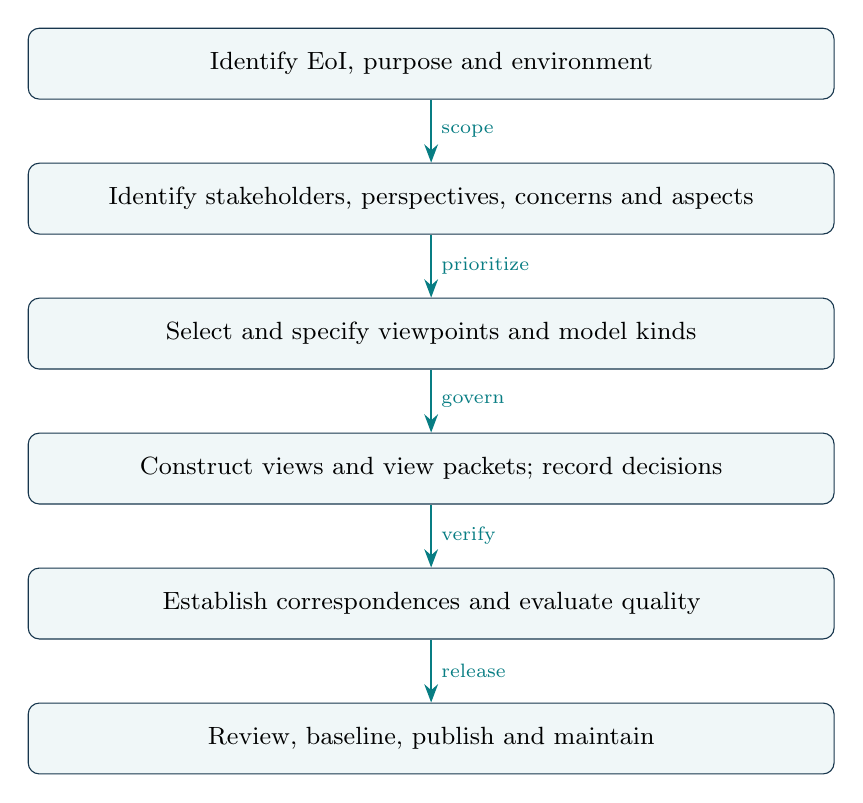
\begin{tikzpicture}[n/.style={draw=navy,rounded corners,fill=teal!6,text width=10cm,align=center,minimum height=9mm,font=\small},>=Stealth]
\node[n] (n0) {Identify EoI, purpose and environment};
\node[n,below=8mm of n0] (n1) {Identify stakeholders, perspectives, concerns and aspects};
\node[n,below=8mm of n1] (n2) {Select and specify viewpoints and model kinds};
\node[n,below=8mm of n2] (n3) {Construct views and view packets; record decisions};
\node[n,below=8mm of n3] (n4) {Establish correspondences and evaluate quality};
\node[n,below=8mm of n4] (n5) {Review, baseline, publish and maintain};
\draw[->,teal,thick] (n0) -- node[right,font=\scriptsize] {scope} (n1);
\draw[->,teal,thick] (n1) -- node[right,font=\scriptsize] {prioritize} (n2);
\draw[->,teal,thick] (n2) -- node[right,font=\scriptsize] {govern} (n3);
\draw[->,teal,thick] (n3) -- node[right,font=\scriptsize] {verify} (n4);
\draw[->,teal,thick] (n4) -- node[right,font=\scriptsize] {release} (n5);\end{tikzpicture}\end{center}
The flow is iterative, not a standards-mandated process. Early viewpoints can be selected provisionally; refine them when stakeholder questions or architectural evidence change. At baseline, every referenced view and model kind must resolve to an identified version.

\begin{longtable}{@{}>{\RaggedRight\arraybackslash}p{0.457\linewidth}>{\RaggedRight\arraybackslash}p{0.457\linewidth}@{}}
\toprule
\textbf{Phase} & \textbf{Work and exit evidence}\\\midrule
\endhead
1. Scope & Record EoI, environment, purpose, baseline, limits and prior evaluation findings. Exit: agreed scope.\\
2. Elicit & Interview roles; express concerns as questions; identify perspectives and aspects. Exit: mapped register.\\
3. Select & Build concern-to-viewpoint matrix; merge overlapping candidates only when semantics remain clear. Exit: coverage and rationale.\\
4. Specify & Define types, relations, legends, view and correspondence methods. Exit: versioned viewpoint catalog.\\
5. Describe & Gather evidence; build models, views, interfaces and behavior; record issues. Exit: readable packets.\\
6. Reconcile & Map modules to runtime elements and deployment nodes; record rule outcomes and violations. Exit: correspondence register.\\
7. Evaluate & Walk through quality scenarios, trade-offs and constraints. Exit: evidence, findings and owners.\\
8. Baseline & Perform separate document quality and normative assessment; approve scope and version. Exit: release and change triggers.\\
\bottomrule
\end{longtable}
\docsection{Selecting structures and views}
V\&B chapters 1--5 organize architectural structures into module, component-and-connector (C\&C), and allocation families. Select views by stakeholder need rather than drawing every available style. Use a simple set-cover analysis: prioritize high-impact concerns, select candidates, verify coverage, then remove redundant views if all relevant questions still have adequate answers. Record selection rationale and deliberately omitted views.

\begin{longtable}{@{}>{\RaggedRight\arraybackslash}p{0.297\linewidth}>{\RaggedRight\arraybackslash}p{0.297\linewidth}>{\RaggedRight\arraybackslash}p{0.297\linewidth}@{}}
\toprule
\textbf{Family} & \textbf{Questions} & \textbf{Representative styles}\\\midrule
\endhead
Module & What implementation units exist? How are dependencies constrained? & Decomposition, uses, generalization, layers, aspects, data model.\\
C\&C & What executes? How do units interact, fail and scale? & Pipe/filter, client-server, peer-to-peer, service-oriented, publish-subscribe, shared data.\\
Allocation & Where do units execute, install or get developed? & Deployment, install, work assignment.\\
\bottomrule
\end{longtable}
A module is not necessarily a runtime component. One implementation module can realize multiple component instances; one component can use several modules. Allocation maps software onto execution, file-system or organizational structures. Security and behavior can cut across all three families. A hybrid diagram is useful only when its types and relations remain unambiguous.

\docsection{View packets and beyond-view information}
Adapt V\&B section 10.1 to each view: a primary presentation, catalog of elements and relations with their properties, interfaces and behavior, context, variability, and rationale. Partition large views into packets with navigable parent-child links. Use stable identifiers instead of repeating conflicting facts. Each packet identifies scope and baseline, governing viewpoint, model kind or legend, assumptions, and known issues.

\begin{longtable}{@{}>{\RaggedRight\arraybackslash}p{0.457\linewidth}>{\RaggedRight\arraybackslash}p{0.457\linewidth}@{}}
\toprule
\textbf{Packet section} & \textbf{Content and verification}\\\midrule
\endhead
Primary presentation & Diagram/table with typed relationships, boundary and legend; resolve every referenced ID.\\
Catalog & Element purpose, type, responsibility, properties; connector semantics and constraints.\\
Interfaces and behavior & Contracts, errors, concurrency, interaction traces, state transitions and failure cases.\\
Context & External actors and interfaces, what is excluded and assumptions.\\
Variability & Permitted choices, conditions, extension points, prohibited variants.\\
Rationale & Why the structure was chosen; linked decisions and alternatives.\\
Known issues & Open risks, deviations and inconsistency references; owner and next review.\\
\bottomrule
\end{longtable}
V\&B section 10.2 places information used by multiple views outside individual views: documentation roadmap, conventions for reading views, overview, mappings between views, shared rationale and an element directory. Add quality scenarios, security assumptions and evidence references when they span multiple views. A shared view component can be reused across views without duplication under ISO 42010 clause 6.8.

\docsection{Modeling conventions and evidence}
Choose a model kind for each modeled view component. Specify syntax, meaning, allowed element types, relationships, constraints, creation and analysis methods, and version. A UML package dependency is not automatically a V\&B uses relation; declare the semantics. For non-model-based text, identify its legend and conventions. Avoid unnamed arrows, unexplained icons or diagrams where a relationship changes meaning midstream.

\begin{longtable}{@{}>{\RaggedRight\arraybackslash}p{0.457\linewidth}>{\RaggedRight\arraybackslash}p{0.457\linewidth}@{}}
\toprule
\textbf{Convention} & \textbf{Local rule}\\\midrule
\endhead
Identity & Use stable IDs STK, PER, CON, ASP, VP, MK, V, VC, M, C, N, COR, CM, ADR, QAS, EV and ISSUE. Do not recycle IDs.\\
Relation semantics & State direction, cardinality and type; distinguish runtime calls from dependency and deployment.\\
Baseline & Record source commit or design revision, observation date and whether inferred or observed.\\
Provenance & Evidence records name artifact, version, locator, author/reviewer, verification outcome.\\
Abstraction & Declare what the diagram suppresses; distinguish types from instances; use view packets.\\
Unknowns & Use unknown, proposed or not verified explicitly; never fill an evidence gap with assumption.\\
\bottomrule
\end{longtable}
Example: a dependency graph recovered from imports may not capture reflection, plugins or generated runtime wiring. Record the extraction method, then reconcile with configuration and traces. A rendered diagram proves syntax was accepted by a renderer, not the correctness of its semantic claims.

\docsection{Traceability and consistency}
\begin{center}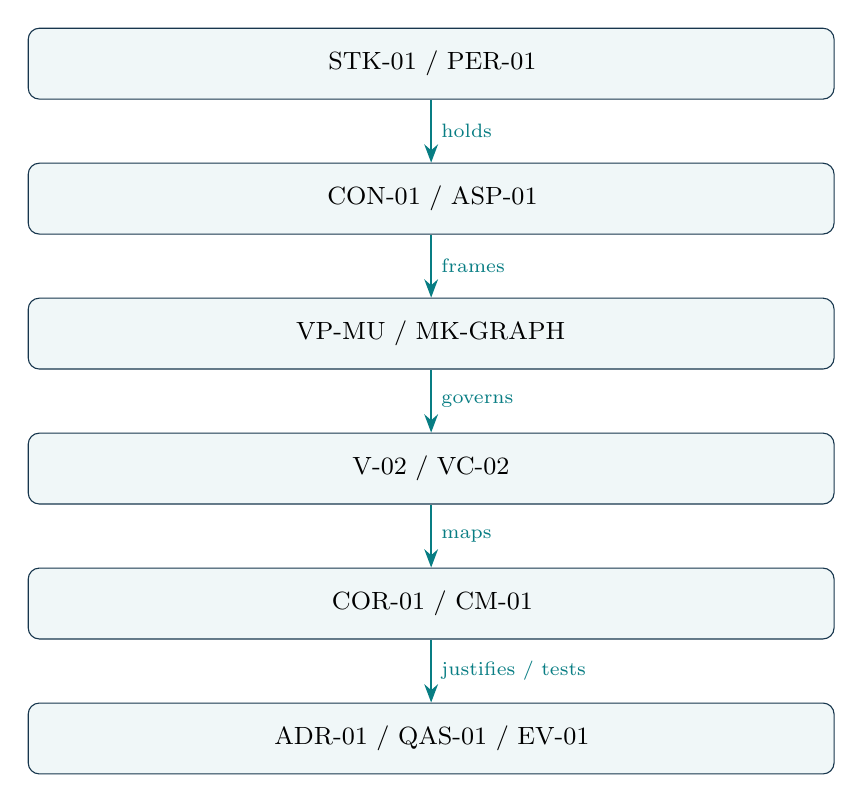
\begin{tikzpicture}[n/.style={draw=navy,rounded corners,fill=teal!6,text width=10cm,align=center,minimum height=9mm,font=\small},>=Stealth]
\node[n] (n0) {STK-01 / PER-01};
\node[n,below=8mm of n0] (n1) {CON-01 / ASP-01};
\node[n,below=8mm of n1] (n2) {VP-MU / MK-GRAPH};
\node[n,below=8mm of n2] (n3) {V-02 / VC-02};
\node[n,below=8mm of n3] (n4) {COR-01 / CM-01};
\node[n,below=8mm of n4] (n5) {ADR-01 / QAS-01 / EV-01};
\draw[->,teal,thick] (n0) -- node[right,font=\scriptsize] {holds} (n1);
\draw[->,teal,thick] (n1) -- node[right,font=\scriptsize] {frames} (n2);
\draw[->,teal,thick] (n2) -- node[right,font=\scriptsize] {governs} (n3);
\draw[->,teal,thick] (n3) -- node[right,font=\scriptsize] {maps} (n4);
\draw[->,teal,thick] (n4) -- node[right,font=\scriptsize] {justifies / tests} (n5);\end{tikzpicture}\end{center}
This chain is a reading aid, not a mandatory linear relationship. Maintain many-to-many records: stakeholder-perspective-concern, concern-aspect, perspective-viewpoint, concern-viewpoint, viewpoint-view, view-component and cross-view relations. An architecture decision links to the affected concerns and elements; a quality scenario tests a claim and does not become architecture merely by association.

\begin{longtable}{@{}>{\RaggedRight\arraybackslash}p{0.297\linewidth}>{\RaggedRight\arraybackslash}p{0.297\linewidth}>{\RaggedRight\arraybackslash}p{0.297\linewidth}@{}}
\toprule
\textbf{Method} & \textbf{Local validation} & \textbf{Failure handling}\\\midrule
\endhead
CM-01 realizes & Each in-scope runtime component maps to one or more modules or an identified external artifact. & Record missing source mapping and owner.\\
CM-02 deployed-on & Every deployable runtime instance has a target in selected environment. & List unmapped component or environment exception.\\
CM-03 covers & Every identified concern, perspective and aspect has actual view coverage; viewpoint framing alone is insufficient. & Create missing view content or record nonconformance.\\
CM-04 contract & Each modeled connector references an interface with compatible protocol and direction. & Identify conflicting endpoint and update contract.\\
CM-05 decision & Each essential decision has rationale; affected elements resolve. & Block local release until rationale or defect is recorded.\\
\bottomrule
\end{longtable}
For each applied correspondence method record whether it holds or the known violations; identify participating ADs, elements and method in correspondence records. Do not label a missing relation as passed simply because a diagram looks consistent. Preserve unresolved inconsistencies explicitly (ISO 42010 6.9).

\docsection{Quality attributes and decision rationale}
Convert important concerns into stimulus-response scenarios: source, stimulus, environment, affected artifact, response and measurable response criterion. Distinguish a target from a measured result. Use simulations, review, load tests, fault injection or threat modeling when appropriate. Keep the evidence with the architecture baseline; record assumptions and untested claims.

\begin{longtable}{@{}>{\RaggedRight\arraybackslash}p{0.297\linewidth}>{\RaggedRight\arraybackslash}p{0.297\linewidth}>{\RaggedRight\arraybackslash}p{0.297\linewidth}@{}}
\toprule
\textbf{Concern} & \textbf{Illustrative criterion} & \textbf{Evidence}\\\midrule
\endhead
Reliability & After a worker loss, accepted jobs are recovered within 5 minutes; duplicate results are not published. & Fault test and result log.\\
Security & Unauthorized callers cannot start privileged actions. & Negative authorization and boundary tests.\\
Modifiability & Adding a provider adapter requires no domain-core changes. & Dependency rule and change exercise.\\
\bottomrule
\end{longtable}
An ADR records context, decision, status, alternatives, rationale, consequences, affected IDs, assumptions and revisit trigger. ISO clause 6.10 requires rationale for essential decisions; recording alternatives and viewpoint selection rationale is recommended. A decision to accept a risk does not by itself demonstrate conformance or operational safety.

\docsection{Documentation lifecycle and governance}
Maintain sources under version control; assign owners for viewpoints, views and decisions. Review when dependencies, interfaces, deployment topology, threat assumptions, quality targets, ownership or major constraints change. Version related evidence with the documented baseline. Use change requests that identify affected views and correspondences, then rerun checks. A docs-only change may still require technical reviewer approval.

\begin{longtable}{@{}>{\RaggedRight\arraybackslash}p{0.457\linewidth}>{\RaggedRight\arraybackslash}p{0.457\linewidth}@{}}
\toprule
\textbf{Gate} & \textbf{Criteria}\\\midrule
\endhead
Author & All referenced identifiers resolve; distinction between observed and proposed state.\\
Architecture & Semantics, coverage, alternatives, rationale and consistency inspected.\\
Stakeholder & Concern owners confirm that the representation answers intended questions.\\
Conformance & Clause-level evidence reviewed for the claimed object; no hidden tailoring.\\
Publication & Build passes, links and diagrams render, private evidence and licensed source material excluded.\\
\bottomrule
\end{longtable}
Use the companion template and printable blank for project adoption; the catalog for reusable viewpoint definitions; the conformance guide for standards evidence; the checklist for structured review; the reference AD for a worked example. This package does not replace domain-specific design analysis.

\docsection{Source register and scope}
\begin{enumerate}
\item ISO/IEC/IEEE 42010:2022, \emph{Software, systems and enterprise --- Architecture description}, second edition, November 2022. Supplied licensed copy consulted; citations refer to clause numbers, not PDF pagination. Official record: \url{https://www.iso.org/standard/74393.html}.
\item P. Clements et al., \emph{Documenting Software Architectures: Views and Beyond}, second edition, Addison-Wesley, 2011, ISBN 978-0-321-55268-6. Supplied copy consulted; citations refer to book chapters and sections.
\end{enumerate}
All procedures, examples, record identifiers, tables, and proposed engineering controls in this suite are original implementation guidance. Neither source is redistributed. The book predates the 2022 edition; its historical standards comparison is not evidence of compliance with the later edition. Consult the actual standard for normative wording and applicability. This suite is not certification, legal advice, or a substitute for independent architecture evaluation.
\end{document}
